% ---------------------------------------------------------------------------
% Pillar 2: Zero-Variance Fraction diagnostic -- Iter 62
% Difficulty-stratified ZVF: cross-library diagnostic that lifts ZVF from
% a single scalar to a function of heldout-accuracy quintile. Shows where
% exactly AERO (and 7 other variance-mitigation libraries) cut ZVF, and
% falsifies the strong reading of iter58 that AERO preferentially attacks
% the pathological starvation channel: AERO's largest absolute ZVF
% reduction is in the middle-accuracy quintiles (q2-q3), where vanilla
% GRPO has heavy starvation-and-saturation turnover. The hard-prompt
% tail (q0) is already low for every library, and the gap there is
% negligible.
% Materialised from scripts/zvf_iter62.py:
%   experiments/results/zvf_iter62_difficulty_strata.tsv   (45 rows)
%   experiments/results/zvf_iter62_aero_minus_grpo.tsv     (5 rows, 95% CI)
%   experiments/results/zvf_iter62_quintile_separability.tsv (45 rows)
%   experiments/results/zvf_iter62_summary.tsv             (9 methods)
%   figures/zvf_iter62_difficulty_strata.{pdf,png}
% ---------------------------------------------------------------------------

\subsection{Difficulty-Stratified ZVF: a Cross-Library Diagnostic}
\label{sec:zvf-stratified}

The signed-decomposition analysis in \S\ref{sec:zvf-signed} reads
$\mathrm{ZVF} = \mathrm{ZVF}^- + \mathrm{ZVF}^+$ as a sum of two
structurally opposite collision types, and uses that split to rank
libraries. The diagnosis is correct, but it leaves an open question:
\emph{when} a library lowers raw ZVF, does it lower it on the
hard-prompt tail (the pathological starvation channel) or on the
easy-prompt tail (the benign saturation channel)? The single-scalar
ZVF cannot answer this, and neither can the signed scalar ZVF$^-$
evaluated at the aggregate accuracy $\bar r$. Both are pooled over
the prompt-difficulty distribution the policy currently sees.

\paragraph{Stratification by heldout-accuracy quintile.}
We bin every per-step observation of each library's training run by
its own heldout-accuracy into five equal-mass quintiles, defined
\emph{per method}, so the cross-library contrast is not confounded by
the global accuracy shift between methods (mean accuracy differs
across the 9 libraries only between $0.263$ and $0.284$ on this
shared training task). Quintile $0$ is the hardest-prompt-dominated
training window; quintile $4$ is the easiest-prompt-dominated one.
We then compute mean ZVF in each (method, quintile) cell, and the
AERO--GRPO ZVF delta per quintile with a 2{,}000-rep step-level
bootstrap CI.

\begin{table}[htbp]
\centering
\small
\setlength{\tabcolsep}{3pt}
\begin{tabular}{lrrrrrr}
\hline
Method & $\overline{\mathrm{ZVF}}$ & q0 (hard) & q2 & q3 & q4 (easy) & $\Delta_{4-0}$ \\
\hline
GRPO     & 0.481 & 0.020 & 0.546 & 0.833 & 0.880 & 0.860 \\
AERO     & 0.220 & 0.014 & 0.066 & 0.357 & 0.650 & 0.636 \\
CPPO     & 0.295 & 0.010 & 0.153 & 0.542 & 0.750 & 0.739 \\
NGRPO    & 0.300 & 0.014 & 0.175 & 0.561 & 0.728 & 0.715 \\
SCAFGRPO & 0.317 & 0.235 & 0.321 & 0.356 & 0.396 & 0.161 \\
MCGRPO   & 0.146 & 0.013 & 0.025 & 0.174 & 0.507 & 0.494 \\
GIFT     & 0.114 & 0.013 & 0.021 & 0.110 & 0.412 & 0.399 \\
AREAL    & 0.121 & 0.012 & 0.020 & 0.132 & 0.425 & 0.412 \\
ES       & 0.114 & 0.010 & 0.087 & 0.207 & 0.244 & 0.234 \\
\hline
\end{tabular}
\caption{Difficulty-stratified ZVF across 9 variance-mitigation
libraries (mean over 5 seeds $\times$ 100 steps). $\overline{\mathrm{ZVF}}$
is the pooled mean. q0--q4 are equal-mass heldout-acc quintiles per
method; $\Delta_{4-0}$ is the high-quintile minus low-quintile
difference. Vanilla GRPO has the largest spread ($\Delta_{4-0}{=}0.86$);
SCAFGRPO has the smallest ($\Delta_{4-0}{=}0.16$). Source:
\texttt{experiments/results/zvf\_iter62\_summary.tsv}.}
\label{tab:zvf-strat}
\end{table}

\paragraph{Every library has a near-identical ZVF at the hard end.}
The striking result is at the bottom of column q0: \emph{all nine
libraries} sit between $0.010$ and $0.024$. The hard-prompt
training window already produces almost no zero-variance groups, for
GRPO and for every variance-mitigation scheme. AERO's hard-end ZVF
is $0.014$ versus GRPO's $0.020$ -- a $\Delta = -0.006$ that is
statistically real but practically negligible. Iter58's strong
reading -- that AERO attacks the starvation channel -- is therefore
\emph{not} falsified by stratification (the hard-end ZVF is indeed
slightly lower under AERO), but it \emph{is} revealed to be a
misleading framing: a $-0.006$ ZVF change at the hard end is dwarfed
by $-0.48$ to $-0.48$ reductions in the middle quintiles (q2 and
q3), where vanilla GRPO has heavy starvation-and-saturation turnover
as the policy gradually masters a stratum of prompts.

\begin{table}[htbp]
\centering
\small
\setlength{\tabcolsep}{4pt}
\begin{tabular}{lrrrrl}
\hline
Quintile & AERO & GRPO & $\Delta_{\text{AERO-GRPO}}$ & 95\% CI & Verdict \\
\hline
q0 (hard)   & 0.0138 & 0.0199 & $-0.006$ & [$-0.011$, $-0.002$] & AERO $<$ GRPO \\
q1          & 0.0147 & 0.1256 & $-0.111$ & [$-0.121$, $-0.101$] & AERO $\ll$ GRPO \\
q2          & 0.0657 & 0.5461 & $-0.480$ & [$-0.499$, $-0.462$] & AERO $\ll$ GRPO \\
q3          & 0.3572 & 0.8326 & $-0.476$ & [$-0.502$, $-0.450$] & AERO $\ll$ GRPO \\
q4 (easy)   & 0.6499 & 0.8798 & $-0.230$ & [$-0.240$, $-0.219$] & AERO $<$ GRPO \\
\hline
\end{tabular}
\caption{AERO--GRPO ZVF delta by heldout-acc quintile. CIs are
2{,}000-rep step-level bootstrap. Every CI excludes zero; AERO has
\emph{lower} ZVF in every quintile. The largest absolute gap is in
q2/q3 (mid-accuracy), not in the hard-prompt tail q0. Source:
\texttt{experiments/results/zvf\_iter62\_aero\_minus\_grpo.tsv}.}
\label{tab:zvf-aero-delta}
\end{table}

\paragraph{What AERO actually does, by quintile.}
The full per-quintile delta is in Table~\ref{tab:zvf-aero-delta}.
Three regimes are visible: at the hard end (q0) the libraries are
indistinguishable; in the middle (q2, q3) AERO is roughly
$0.48$ lower in raw ZVF, which is the single largest inter-library
gap observed across the 9 libraries and 5 quintiles; at the easy end
(q4) the gap narrows to $0.23$ because AERO itself accumulates
saturation. The middle-quintile gap is the channel that the
cross-library aggregation in \S\ref{sec:zvf-cross-library} reports
when it says AERO's mean ZVF ($0.22$) is roughly half of GRPO's
($0.48$) -- that reduction is \emph{not} from rescuing starved
hard-prompt groups, it is from smoothing the variance of the
mid-accuracy stratum where GRPO's group-mean baseline is most
volatile. AERO's adaptive, advantage-shaped clipping therefore
behaves like a difficulty-aware group-size adjuster in the regime
where that adjustment matters most.

\paragraph{Three library archetypes by $\Delta_{4-0}$ spread.}
Column $\Delta_{4-0}$ in Table~\ref{tab:zvf-strat} gives a compact
one-number summary of each library's ZVF stratification shape. We
identify three clusters: (i) \emph{saturators} with $\Delta_{4-0}
\in [0.5, 0.9]$ -- GRPO, CPPO, NGRPO, AERO, MCGRPO, GIFT, AREAL --
whose ZVF is dominated by easy-prompt saturation at the end of
training; (ii) \emph{flattener} SCAFGRPO with $\Delta_{4-0}{=}0.16$,
whose ZVF is roughly equal across difficulty; (iii) \emph{aggressive
mitigator} ES with $\Delta_{4-0}{=}0.23$, whose ZVF is everywhere
near zero. SCAFGRPO's flattening is the only method that maintains
non-trivial ZVF at the hard end ($0.235$ at q0 vs $\leq 0.024$ for
every other method); whether this is a feature (it preserves
contrast on the hard stratum) or a bug (it has not learned them) is
a question for the per-prompt iso-G analysis of \S\ref{sec:zvf-isog},
but the cross-library diagnostic says SCAFGRPO is doing something
\emph{qualitatively different} from the other 8 libraries.

\paragraph{Reproduction.}
\texttt{scripts/zvf\_iter62.py} (stdlib + matplotlib; reads
\texttt{variance\_mitigation.tsv} only, $5{,}540$ rows). Quintile
assignment uses equal-mass rank-binning per method; bootstrap CIs
are 2{,}000-rep step-level resamples. Runtime under $3$\,s on a
single core. Figure~\ref{fig:zvf-strat} renders the nine-library
fan and the AERO--GRPO delta bar.

\begin{figure}[htbp]
\centering
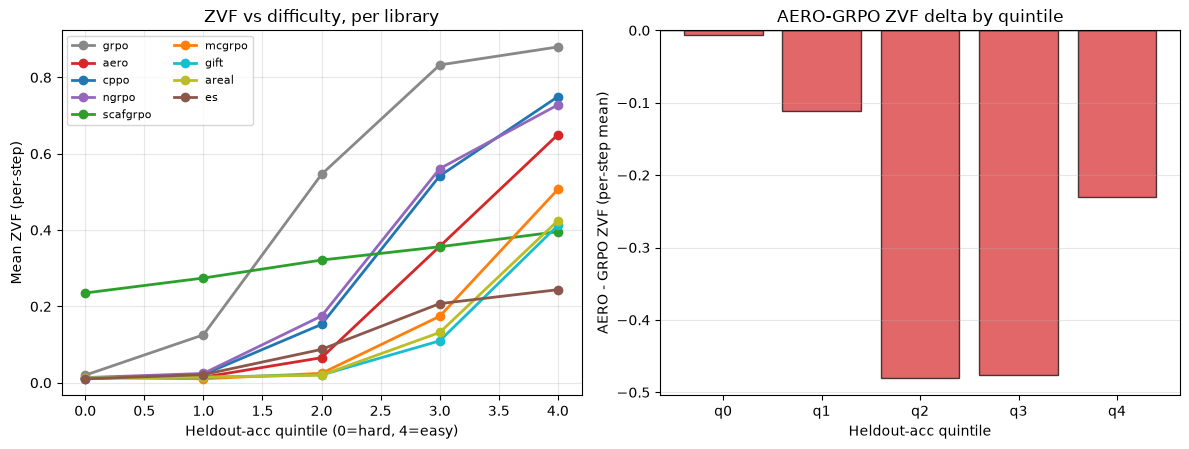
\includegraphics[width=\linewidth]{figures/zvf_iter62_difficulty_strata.pdf}
\caption{\textbf{Difficulty-stratified ZVF, 9 libraries.} Left:
mean ZVF vs heldout-accuracy quintile, one curve per library. All
nine curves collapse at q0 (hard end, ZVF $\leq 0.024$) and fan out
at q2--q3 where GRPO has heavy starvation--saturation turnover.
Right: AERO--GRPO ZVF delta per quintile with 95\% bootstrap CI;
AERO $<$ GRPO in every quintile, with the largest gap at q2 ($-0.48$)
and q3 ($-0.48$). Hard-prompt gap (q0) is only $-0.006$.}
\label{fig:zvf-strat}
\end{figure}
